\chapter{In Media We ... Trust?}

Despite the news media ecosystem's rapid evolution in the past decade, the question of fairness in reporting remains a valued one. Although counterarguments for subjective reporting exist (Glenn Greenwald, most famous for his coverage of whistleblower Edward Snowden's leaks, said that ``All journalism is a form of activism. Every journalistic choice necessarily embraces highly subjective assumptions--cultural, political or nationalistic--and serves the interests of one faction or another''), fair treatment of subjects and sources remain a central tenant to most publications \cite{Greenwald}. 
  
But an attempt at fairness on the side the reporter is not always perceived in equal effect under the eyes of the reader. Presenting contradictory facts to a reader's beliefs can even sometimes \emph{strengthen} their oppositions to it, a concept known as ``motivated skepticism'' \cite{taber2006motivated}.

In this section, we examine the impact of distrust in media, and explore the theories behind three main potential sources of media distrust: the characteristics of the reader, the source of the story and its use of language.

% In evolving news ecosystem, question of fairness is highly valued in the press. Most news publications have some stipulation of fairness in their handbook.
% See: Nieman Report [http://niemanreports.org/articles/fairness-in-journalism-is-rewarded/]
% Handbooks (Reuters: http://handbook.reuters.com/?title=Freedom_from_bias, NPR, etc.)

% History of press fairness: Fairness Doctrine of 1949
  
\section{Why Does Media Trust Matter?} 
 
 The idea that mass media has a large influence on the ramifications of democracy is nothing new. In 1922, political commentator, reporter, and writer Walter Lippman wrote about its central role in shaping public opinion:

     \begin{quote}Each of us lives and works on a small part of the earth's surface, moves in a small circle, and of these acquaintances knows only a few intimately. Of any public event that has wide effects we see at best only a phase and an aspect. This is as true of the eminent insiders who draft treaties, make laws, and issue orders, as it is of those who have treaties framed for them, laws promulgated to them, orders given at them. Inevitably our opinions cover a bigger space, a longer reach of time, a greater number of things, than we can directly observe. They have, therefore, to be pieced together out of what others have reported and what we can imagine.
    Yet even the eyewitness does not bring back a naive picture of the scene. 
    \cite{lippman1922public} 
    \end{quote} 

Many of the worries that Lippman had about the effects of poorly disseminated truth have been later confirmed in experimental studies. In short, when faced with a large and mistrusted news environment, we tend to rely on \emph{confirmation bias} when searching for information. This term, first coined in 1988, describes the psychological phenomeon of seeking or analyzing new information in ways that align with one's existing beliefs, expectations or prior hypotheses \cite{nickerson1998confirmation}.

Using a Bayesian voting model, a study from Georgetown University in 2005 was able to show that voters with low trust and a high dislike for the news media are significantly more influenced by their existing party identifications in casting ballots than current economic factors \cite{ladd2005attitudes}. The study attributes increasing polarization in the American political sphere with increasing lack of trust in the news, a serious implication for the highly polarized 2016 presidential elections. Moreover, distrust of media implies a large information loss in the public, whose avoidance of diverse ideas means a narrowing of information flow \cite{ladd2011americans}.  

%How can reading a diverse array of news be good? 
\section{How is Media Trust Formed?}
\subsection{The Role of the Reader}

% In this section:
%% Hostile Media (1985)
%% Gunther, Curvlinear (1988)
%% The Liberal Media Myth Revisited (2005)
% Transition into next section: well, of course, it's not just one big media...
The perception of media bias is a cornerstone component of distrust in the news. 
After all, most Americans claim that they want to read news that's unbiased. A survey from Pew Research in 2012 showed that more than two-thirds (68\%) of readers want to read political articles with a neutral stance, compared to just a little less than a quarter (23\%) of those who want to read those stories that share their point of view \cite{Pew-bias-2012}. But what exactly does that entail?

It comes as no surprise that our own political stances have a significant effect in our perceptions of bias in the media. On whole, conservative readers tend to view media as more biased than both Democrats and Independents (49\% to 32\% and 35\%, respectively)\cite{Pew-bias-2012}. Partisans have also been shown to view the news as antagonistic to their beliefs, a phenomenon known as the ``hostile media effect''.

The effect, first studied in the 1980s, showed that when faced with the same piece of news media about the Sabra and Shatila massacre in Beirut, pro-Israeli and pro-Palestinian students both claimed the news clip was biased in favor of the other side 
 \cite{vallone1985hostile}. It has since been repeated in a variety of contexts to the same effect.

What the story is reporting does not matter so much as the individual's attitude \emph{towards} that issue. In 1988, Albert Gunther found a curvlinear effect between the viewer's polarization towards an issue and their trust in the media to fairly cover it \cite{gunther1988attitude}. In doing so, he suggests two models of persuasion to help understand media processing: first, the cognitive response theory, which predicts more portential for attitude change when the reader is highly involved in the content, as they are processing information more deeply \cite{cacioppo1979effects}. Social judgement theory, on the other hand, expects less change in attitude when the reader is highly involved or polarized about a subject, as they will simply reject the new information \cite{sherif1961social}. These two opposing theories help explain the presence of a curvlinear relationship to exposure to news media and resulting media trust.

%http://www.niemanlab.org/2012/06/how-do-you-tell-when-the-news-is-biased/
%the cool experiment
 
% Perceptions of media bias, then, have as much to do as self-serving motivations to secure preferential treatment as they do with the media itself. 

\subsection{The Role of Media Brands}

The media, of course, is not just one unified mass, and in an increasingly fragmented ecosystem, the role of brands is a crucial factor in media trust. With the rise of the Internet, the past decade has seen an explosion of new media platforms and publications, as well as significant transformations in style and audience in existing outlets.

Although the studies above present the media as one unified mass, there is a significant amplifying effect of hostility and bias perception depending on the reader's prior connotations of a news outlet. In 2008, researchers Matthew Baum and Phil Gussin showed significant differences in the evaluation of a piece of news content depending on whether it was labeled to be from CNN, Fox, or a fictional news outlet \cite{baum2008eye}. They concluded that media bias is very much ``in the eye of the beholder,'' as viewers make information shortcuts dependent on media brand to jump to conclusions beyond their own partisanship and the content of the story. 

\subsection{The Role of Language}
Finally, the role of language--in media as well as politics--cannot be overlooked. A recent article in the Boston Globe analyzed the language of presidential candidate Donald Trump to be at a fourth grade level-- and more successfully appealing to voters \cite{Globe-language-article}. (Those who have been speaking at lower grade levels in the 2016 election cycle have also been winning more votes.)

Analysis by media outlet Vocativ showed a negative correlation between presidential speech level over time \cite{Vocativ-speech}.

\begin{figure}[h!] 
\centering
  \frame{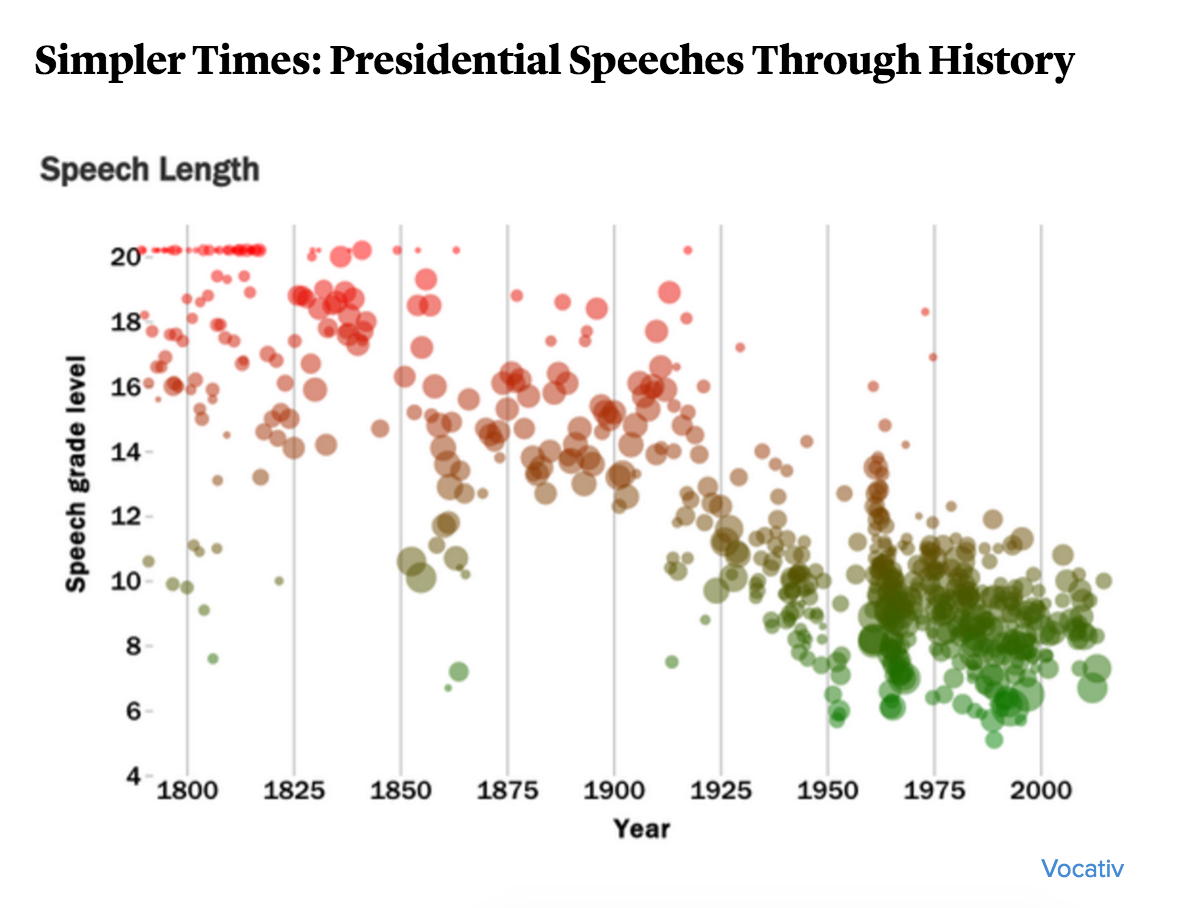
\includegraphics[width=0.8\textwidth]{vocativ_speech}}
  \caption{Language of Presidential Speech Decline}
\end{figure}

Yet political news \emph{coverage} occupies a different space of language and purpose, often with the intent of reporting statistics and facts in a scientific nature using a specified technical vocabulary. And when the reader processes information of a scientific nature, a funny effect has been shown: that more complex language, with more technical jargon and sophisticated construction, might actually \emph{increase} appeal and the likelihood of trust. In 2008, Weisberg et. al showed that the addition of ``neuroscience'' significantly increased the likelihood of believability in explaining how the brain works, versus the same explanation in simple, everyday language \cite{weisberg2008seductive}. These two factors are both at play when considering the impact of the language in political news and its perceived truthworthiness, for the articles are often \emph{both} a reflection of a political candidate as well as its analysis of her or him.




















